

\section{Introduction}
Extracorporeal shock wave therapy (ESWT) is a noninvasive treatment
used to treat musculoskeletal conditions such as bone fractures
that fail to heal (non-unions), necrotic wounds, and strained
tendons.  In this treatment a shock wave is generated in water and
then focused using an acoustic lens or reflector so that the energy
of the wave is concentrated in a small treatment region.  This
technique has been used since the 1980's, more widely in Europe and
Asia than in the US, where it is still considered experimental and
has limited FDA approval.  Although the underlying biological
mechanisms are not well understood \cite{ogden}, the mechanical
stress of cells caused by the propagating shock wave is thought to
initiate the release of substances such as VEGF (vascular endothelial
growth factor) that cause angiogenesis and neo-vascularization, and
hence to increased oxygen supply to damaged tissue, or of similar
osteogenic growth factors in bone.  The medical shock wave devices
are similar to those used for extracorporeal shock
wave lithotripsy (ESWL), a widely-used non-surgical treatment for
kidney stones in which the focused shock waves have sufficient
amplitude to pulverize the kidney stone.  In shock wave therapy the
amplitudes are generally smaller and the goal is mechanical stimulation
rather than destruction, although in some applications such as the
treatment of heterotopic ossifications (see \Sec{ho}) larger
amplitudes may be used.

Figure \ref{fig:hm3_diagram} shows the geometry of a laboratory
shock wave device 
modeled on the clinical Dornier HM3 lithotripter.  The three-dimensional
axisymmetric geometry consists of an ellipsoidal reflector made out
of metal and a cavity filled with water.  A spark plug at the focus
of the ellipse marked F1 generates a bubble which collapses and
creates a spherical shock wave that reflects and focuses at F2.  
The major and minor axes of the
ellipsoid in the HM3 are $a=140$mm and $b=79.8$mm, respectively.
The foci of this ellipse are at $(\pm 115, 0, 0)$ and the reflector
is truncated at $100$mm from F1, or $(-10,0,0)$.  

In the laboratory, this reflector is immersed in a bath of water
and objects can be
placed at the second focus of the ellipsoid, F2.
This device is in use at the Center for Industrial and Medical Ultrasound
(CIMU) at the University of Washington Applied Physics Laboratory and we
have used this geometry in order to compare directly with some laboratory
experiments.

Computationally, we
use this geometry to calculate the initial condition by solving
two-dimensional axisymmetric Euler equations with the Tamman equation of
state (see \Sec{eos}).   These initial conditions are then fed into a full 
three-dimensional calculation near the focus at F2.

\begin{figure}
\begin{center}
a) 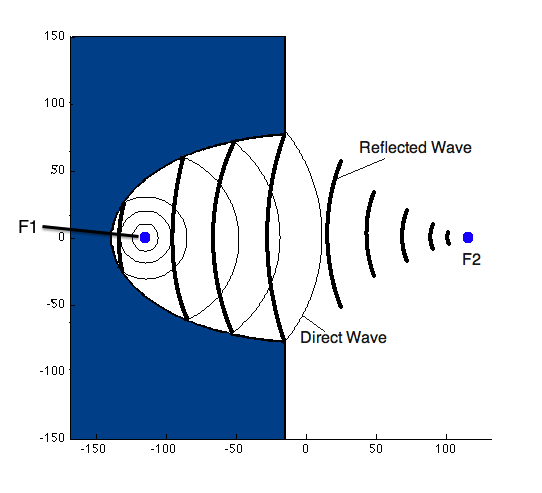
\includegraphics[scale=0.35]{lithotripter_schematic.png}\hspace{1mm}
b) 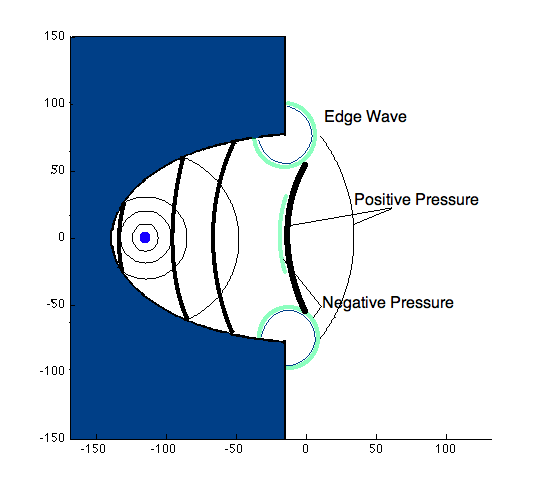
\includegraphics[scale=0.35]{lithotripter_edge_wave.png}
\end{center}
\caption{Cartoon of the Dornier HM3 Lithotripter.  In a) the spherical wave is generated at F1, reflects off the ellipsoid and the reflected wave focuses at F2.  In b) the diagram illustrates the creation of the edge waves at the corner of the ellipsoid and the contribution of negative pressure to the tail of the ESWT pressure wave.}
\label{fig:hm3_diagram}
\end{figure}

In addition to the HM3, we have also used the geometry of the
hand-held Sanywave device used by our collaborator Dr. Michael Chang.
Some sample calculations related to the study of HOs are presented in
\Sec{HO}.

In each case, the ESWT pressure wave form
that is generated has a similar shape. There is a sharp increase
in pressure from atmospheric pressure ($\sim0.1$MPa)
to a peak  pressure ranging from $35--100$
MPa over a very short rise time ($\sim10$ns), 
followed by a decrease in pressure to $\sim-10$
MPa over $\sim5 \mu$s. The negative fluid pressure in the tail can lead to
cavitation bubbles, as discussed below.

%Discuss shock wave profile?

Computational models for shock wave propagation and focusing can
aid in the study of ESWT.  In particular, there are many open
questions concerning the interaction of shock waves with complex
three-dimensional geometries such as bone embedded in tissue.
Because of the difference in material properties, a wave hitting
the tissue/bone interface will be partially reflected, and the
tranmitted wave will have a modified strength and direction of
propagation.  This can greatly affect the location and size of the
focal region as well as the peak pressure amplitude.  Moreover,
although the shock wave is primarily a pressure wave in soft tissue
(which has a very small shear modulus), at a bone interface 
mode conversion takes place and shear waves as well as compressional
waves are transmitted into the bone.  These shear waves may be
important in biological stimulation.  An additional effect is the
formation and collapse of cavitation bubbles that can cause tissue
damage.  While the shock wave is a compression wave, it is followed
by a rarefaction wave of expansion, and in the tail the fluid
pressure typically drops to negative values.  Reflection at interfaces
can lead to enhanced regions of expansion and to sufficiently
negative pressures that cavitation bubbles can form.

To better understand all of these effects, it is desirable to have a
three-dimensional computational model that can simulate the focusing of
nonlinear shock waves and their interaction with arbitrarily complex
interfaces between different materials.  

In this paper we present an approach to this problem that has allowed
the study of some of these issues in a simplified context.  In
particular, we consider an idealized situation in which soft tissue
is replaced by water, ignoring its viscoelastic properties, and
modeled by the nonlinear compressible Euler equations with the
Tamman or Tait equation of state.  Bone is modeled as an isotropic
and homogeneous linear elastic material.

In reality, soft tissue and bone are very complex multiscale materials
with microstructures, inhomogeneities, and anisotropic properties.
Any attempt to model the biological effect of shock wave propagation
through such materials may require a more sophisticated and detailed
model than used here.  However, we believe that many of the macro-scale
shock propagation issues discussed above can be adequately and most
efficiently studied with a simplified model of the form considered here,
since the dominant effect we hope to capture is the reflection and
transmission of waves at interfaces between materials.  

The compressible Euler equations with the Tamman equation of state (see
\Sec{eos_discussion}) in two-dimensional axisymmetric geometry is used to model the
intial formation of the focusing shock wave.  These initial conditions are
then fed into a code that uses a simpler nonlinear
model, the Tait equation of state,
in a three-dimensional simulation of the fluid.  The compressible fluid
equations are written using a Lagrangian formulation that easily couples to
the isotropic linear elasticity equations used in the bone-like material.
The resulting equations have the same form everywhere, with a different
stress-strain relationship in the different materials.

A high-resolution finite volume method is used to solve these equations.
We use the wave-propagation algorithms described in \cite{??}
and implemented in Clawpack \cite{claw.org.url}.  These are Godunov-type
methods for the hyperbolic system that use solutions to the Riemann problem
between adjacent grid cells to determine a set of waves used to update the
solution, and second-order correction terms with slope limiters are added to
resolve the nearly discontinuous shock waves with minimal smearing or
nonphysical oscillation.

These methods are used on a purely rectangular Cartesian grid.  Each
grid cell has associated with it a set of material parameters
determining the material in the cell, in a unified manner so that
both fluid and solid can be modeled.   Complex geometry is handled
by using appropriate averaged values of these parameters in cells
that are cut by the interface.  This is described further in \Sec{??}.
Averaging across the interface works quite well when the material properties
are sufficiently similar and in \Sec{??} we show that this is the case even
for fluid/solid boundaries of the type we consider.  

We also use patch-based adaptive mesh refinement (AMR) to concentrate
grid cells in regions where they are most needed to resolve features
of interest.  The Clawpack software contains AMR software in both
two and three space dimensions and this software has been used
directly for the two-dimensional axisymmetric computations of the
initial shock wave described in \Sec{??}.  For the three-dimensional
problem we have used ChomboClaw \cite{??}, an inteface between
Clawpack and the Chombo code developed at LBL \cite{chomboclaw}, which
provides an implementation of AMR on parallel machines using MPI.
Using ChomboClaw, the code originally developed using Clawpack was
easily converted into a code that was run on a TeraGrid machine at
Texas Advanced Computing Center (TACC) and tested using up to 128 processors.


Extensive laboratory experiments have been performed on
shock wave devices to measure the wave form of shock waves produced by
various devices, the shape of the focal region, the peak amplitudes of
pressure observed in these regions, and other related quantities.  Most of
these experiments have been done in a water tank where the shock wave
propagates and focuses in a homogeneous medium where measurements are easily
done, or with phantoms that are placed in the water as a proxy for bones or
kidney stones, with instrumentation such as pressure gauges or photographs
used to explore the interaction of the shock wave with the object.  In some
cases high-speed photographs of the shock wave have been obtained.
Creating phantoms from clear bi-refringent materials and using polarized
light it is even possible to photograph the shock wave propagating through
the object \cite{??}.  We have used some of these experiments to help
validate our numerical approach (see \Sec{??}).

Other researchers have also developed computational models for 
shock wave therapy and lithotripsy.
In prior work the pressure field has been modeled using linear and
nonlinear acoustics as well as the Euler equations with the Tait
equation of state.  Hamilton \cite{hamilton} used linear geometrical
acoustics, which holds under the assumption of weak shock strength,
to calculate the reflection of the spherical wave.  The diffraction
of the wave at the corner of the reflector was calculated using the
Kirchoff integral method.  Christopher's \cite{christopher_hm3}
model of the HM3 lithotripter used Hamilton's result as a starting
point and considered non planar sources.  Coleman et al \cite{coleman},
Averkiou and Cleveland \cite{cleveland_averkiou} used models based
on the KZK equation.  Tanguay \cite{tanguay} solved the full Euler
equations and incorporated cavitation effects as well as the edge
wave.

Our approach differs from these in that we consider the wave
propagation in both the fluid and solid by solving a single set of
equations that can model both materials.  This approach allows us
to investigate not only compression and tension effects of ESWT,
but also the propagation of shear waves in the solid.  Sapozhnikov
and Cleveland \cite{oleg_cleveland} have investigated the effect
of shear waves on spherical and cylindrical stones using linear
elasticity with a plane wave initial condition.  This initial
condition is an unfocused wave, which yields good results for small
objects, but would fail to capture the full ESWT pressure wave
interaction with three-dimensional bone geometries.

Summary of results in this paper....


